% ============================================================================
% Informe Proyecto #1 -- Computacion Paralela y Distribuida (UVG, Seccion 20)
%
% Fuente reconstruida a partir del PDF original para poder corregirlo.
% Compilar con:  pdflatex informe.tex   (dos veces, por el indice)
% ============================================================================
\documentclass[12pt,letterpaper]{article}

\usepackage[utf8]{inputenc}
\usepackage[T1]{fontenc}
\usepackage[spanish]{babel}
\usepackage[margin=2.5cm]{geometry}
\usepackage{graphicx}
\usepackage{amsmath}
\usepackage{array}
\usepackage{longtable}
\usepackage{booktabs}
\usepackage{pdflscape}
\usepackage{ragged2e}
\usepackage{setspace}
\usepackage[hidelinks]{hyperref}

% Columnas de ancho fijo con texto justificado a la izquierda, para que las
% celdas largas del catalogo de funciones no desborden los bordes.
\newcolumntype{L}[1]{>{\RaggedRight\arraybackslash}p{#1}}
\newcolumntype{M}[1]{>{\RaggedRight\arraybackslash\ttfamily\footnotesize}p{#1}}

\setlength{\parskip}{0.6em}
\setlength{\parindent}{0pt}
\renewcommand{\arraystretch}{1.25}

\begin{document}

% ---------------------------------------------------------------- caratula
\begin{titlepage}
\centering
% parskip a cero: el valor global de 0.6em se suma entre cada \par y empujaba
% los ultimos renglones de la caratula a una segunda pagina.
\setlength{\parskip}{0pt}
\vspace*{1.2cm}
{\Large\bfseries Universidad del Valle de Guatemala\par}
\vspace{0.8cm}
{\large Facultad de Ingeniería\par}
\vspace{0.3cm}
{\large Departamento de Ciencias de la Computación\par}
\vspace{0.3cm}
{\large CC3084 Computación Paralela y Distribuida - Sección 20, Semestre II 2026\par}
\vspace{1.1cm}

\includegraphics[width=0.24\textwidth]{img/logo_uvg.jpg}\par
\vspace{1.0cm}
{\LARGE\bfseries Proyecto \#1\par}
\vspace{1.2cm}
{\bfseries Integrantes del grupo\par}
\vspace{0.5cm}
Roberto Barreda \#23354\par
\vspace{0.25cm}
Nina Najera \#231088\par
\vspace{0.25cm}
José Antón \#221041\par
\vspace{1.2cm}
Guatemala, 2 de septiembre de 2026\par
\end{titlepage}

% ------------------------------------------------------------------ indice
\pagenumbering{roman}
\tableofcontents
\newpage
\pagenumbering{arabic}
\setcounter{page}{1}

% ------------------------------------------------------------ introduccion
\section{Introducción}

El proyecto consiste en el desarrollo de un screensaver basado en una simulación
gravitacional de N cuerpos. Cada cuerpo posee posición, velocidad, aceleración y
masa. Durante cada paso de la simulación, los cuerpos se atraen entre sí y generan
escenas con movimiento continuo.

La solución fue desarrollada en C++ y utiliza SDL2 para mostrar la simulación en
pantalla. También se implementó una versión paralela con OpenMP. El propósito de la
paralelización es distribuir entre varios hilos las operaciones que requieren mayor
tiempo de procesamiento y mejorar el desempeño cuando aumenta la cantidad de cuerpos.

El programa incluye una versión secuencial y una versión paralela construidas a
partir de los mismos archivos fuente. Además, permite configurar la cantidad de
cuerpos, el escenario, el tamaño del canvas, la cantidad de hilos, la semilla
pseudoaleatoria, los parámetros físicos y la política de reparto de OpenMP.

% ------------------------------------------------------------- antecedentes
\section{Antecedentes}

\subsection{OpenMP}

OpenMP es una interfaz de programación paralela orientada a sistemas de memoria
compartida. Permite distribuir trabajo entre varios hilos mediante directivas que se
agregan al código en C y C++. Esto facilita transformar de manera gradual una
solución secuencial en una solución paralela [1].

En este proyecto se utilizan ciclos paralelos para el cálculo de aceleraciones, la
integración del movimiento, el desvanecimiento del framebuffer y otras operaciones
que pueden dividirse entre varios hilos.

\subsection{Simulación de N cuerpos}

Una simulación de N cuerpos representa la interacción entre varios objetos que se
atraen mediante gravedad. En la solución directa implementada, cada cuerpo considera
la influencia de todos los demás. Por esta razón, la cantidad de operaciones crece de
forma cuadrática al aumentar N [3].

La aceleración utilizada en la simulación se expresa como:

\begin{equation}
\vec{a}_i = G \sum_{j} m_j \,
\frac{\vec{r}_j - \vec{r}_i}{\left[ r_{ij}^{2} + \varepsilon^{2} \right]^{3/2}}
\end{equation}

El término $\varepsilon$ corresponde al suavizado de Plummer. Su función es evitar
valores demasiado grandes cuando dos cuerpos se encuentran muy cerca.

Después del cálculo de aceleración se actualizan la velocidad y la posición mediante
Euler semiimplícito:

\begin{align}
\vec{v}_i &\leftarrow \vec{v}_i + \vec{a}_i \, \Delta t \\
\vec{r}_i &\leftarrow \vec{r}_i + \vec{v}_i \, \Delta t
\end{align}

\subsection{Método PCAM}

PCAM divide el diseño de una solución paralela en cuatro etapas: partición,
comunicación, aglomeración y mapeo [2]. Este método es útil para identificar qué
trabajo puede ejecutarse al mismo tiempo y cómo debe distribuirse entre los recursos
disponibles.

La simulación se adapta a este enfoque porque el cálculo de aceleración de un cuerpo
puede realizarse de forma independiente mientras las posiciones de los demás cuerpos
permanezcan sin cambios durante esa fase.

% -------------------------------------------------------------- descripcion
\section{Descripción y funcionamiento del programa}

\subsection{Objetivo de la simulación}

El programa representa cuerpos que se atraen por gravedad y se desplazan de forma
continua dentro de una escena. El movimiento se obtiene directamente de los cálculos
físicos y no de trayectorias dibujadas previamente.

Se implementaron tres escenarios. El modo colisión crea dos galaxias que se aproximan
entre sí. El modo galaxia crea un solo disco en rotación. El modo nube distribuye los
cuerpos de forma pseudoaleatoria y permite observar cómo la gravedad modifica su
distribución.

\subsection{Cumplimiento de los requisitos del screensaver}

\begin{table}[h!]
\centering
\caption{Cumplimiento de los requisitos principales}
\begin{tabular}{|L{4.2cm}|L{9.5cm}|}
\hline
\textbf{Requisito} & \textbf{Implementación} \\
\hline
Cantidad N de elementos & La cantidad de cuerpos se recibe con la bandera
\texttt{-n}. El rango permitido es de 2 a 200000 cuerpos. \\
\hline
Varios colores & Cada cuerpo utiliza una rampa de color combinada con un
desplazamiento pseudoaleatorio generado a partir de la semilla. \\
\hline
Tamaño mínimo del canvas & El ancho mínimo es 640 y el alto mínimo es 480. El valor
predeterminado es 1000 por 700. \\
\hline
Movimiento & La velocidad y la posición de los cuerpos se actualizan en cada paso de
la simulación. \\
\hline
Física y trigonometría & El programa utiliza gravitación, suavizado de Plummer, seno,
coseno y velocidad tangencial para la creación de los discos galácticos. \\
\hline
FPS & El programa calcula y muestra los FPS junto con el tiempo de física y el tiempo
de renderizado. \\
\hline
\end{tabular}
\end{table}

\subsection{Escenario de colisión}

En el modo colisión se crean dos discos galácticos. Cada uno posee un núcleo con
mayor masa y un conjunto de cuerpos distribuidos alrededor de él. Las dos galaxias se
generan con velocidades opuestas y con un desplazamiento que permite observar
deformaciones durante la interacción.

\begin{figure}[h!]
\centering
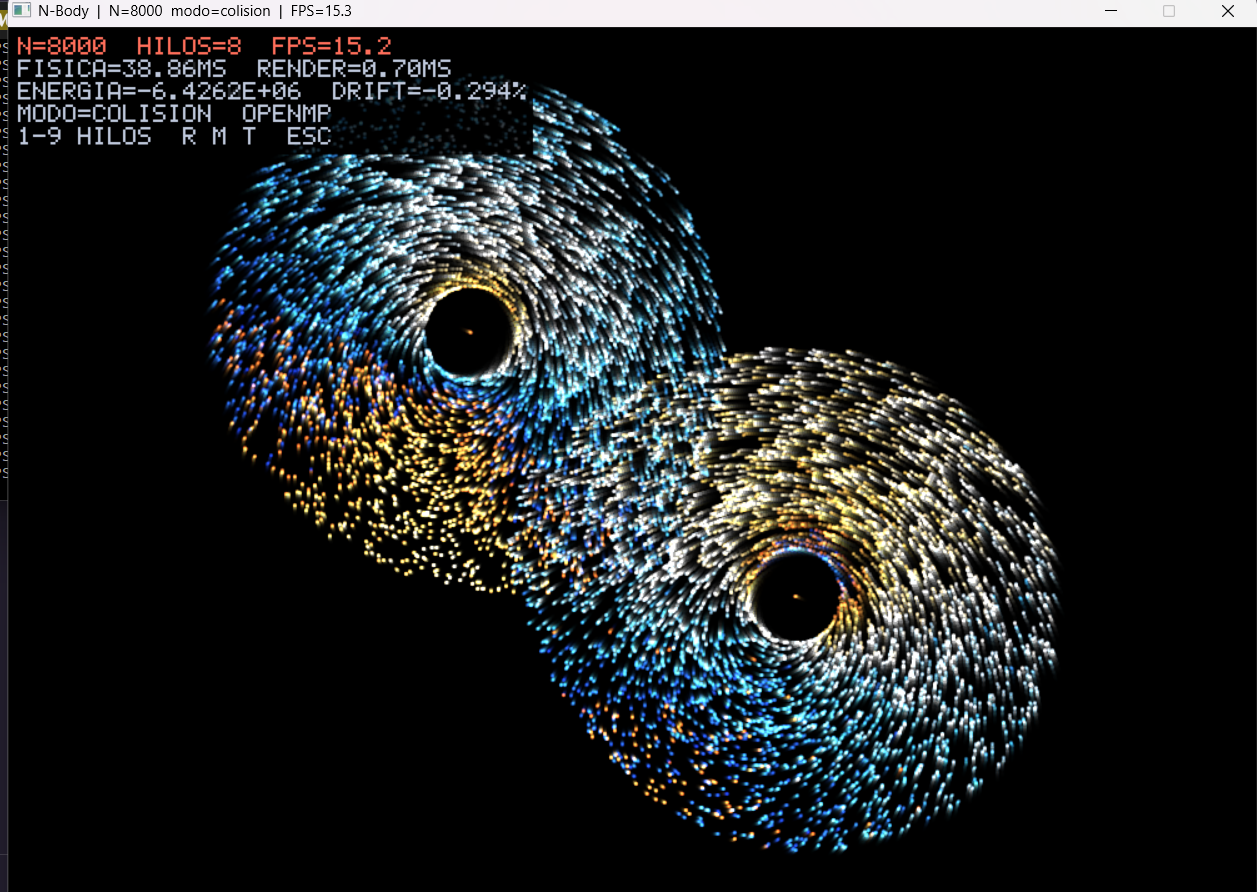
\includegraphics[width=0.85\textwidth]{img/fig1_colision.png}
\caption{Escenario de colisión con 8000 cuerpos y 8 hilos}
\end{figure}

\clearpage
\subsection{Escenario de galaxia}

El modo galaxia genera un solo disco alrededor de un núcleo. Las estrellas reciben una
posición radial y una velocidad tangencial calculada a partir de la masa encerrada
dentro de su radio. Esto produce un patrón de rotación alrededor del centro.

\begin{figure}[h!]
\centering
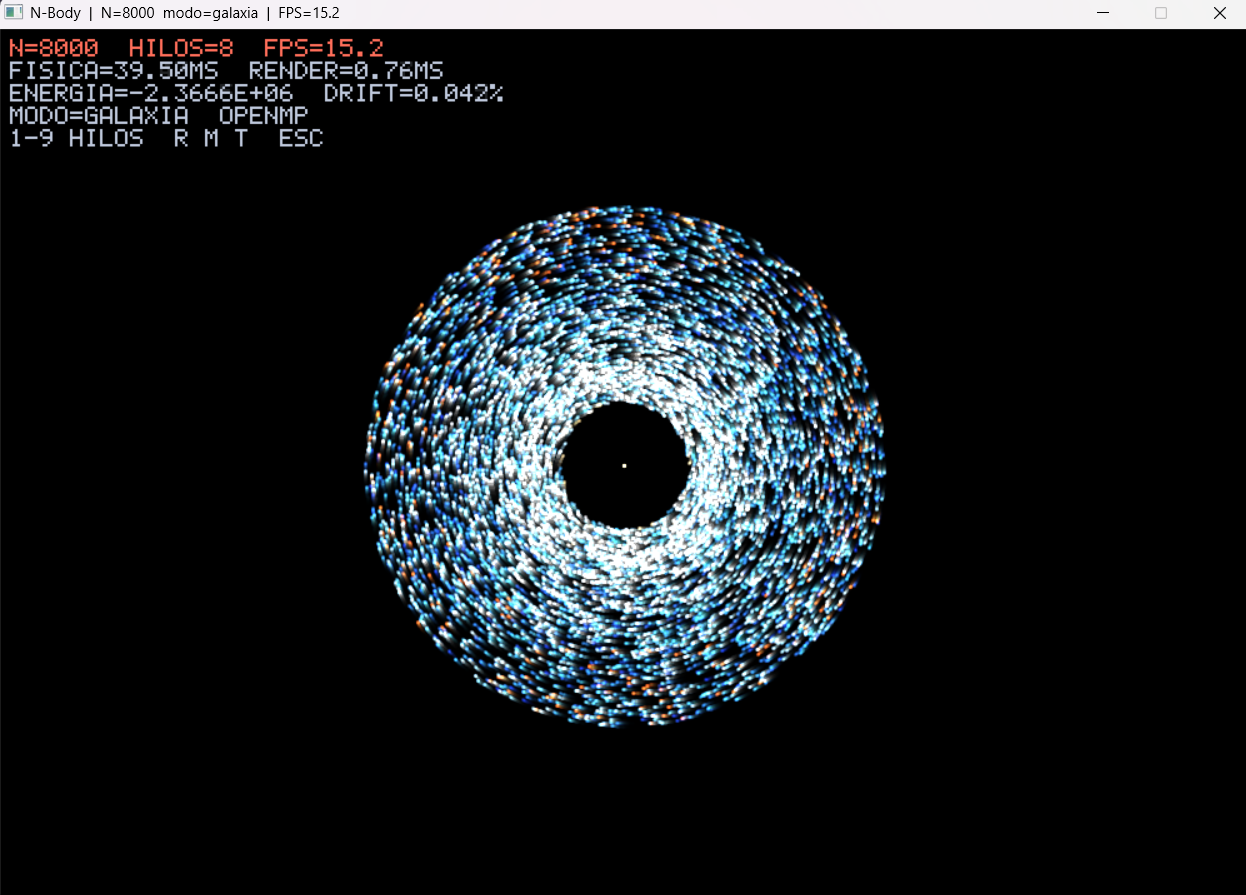
\includegraphics[width=0.85\textwidth]{img/fig2_galaxia.png}
\caption{Escenario de galaxia con 8000 cuerpos y 8 hilos}
\end{figure}

\subsection{Escenario de nube}

El modo nube distribuye cuerpos con masas iguales dentro del canvas. Las velocidades
iniciales son pequeñas y la gravedad modifica progresivamente la forma del conjunto.

\begin{figure}[h!]
\centering
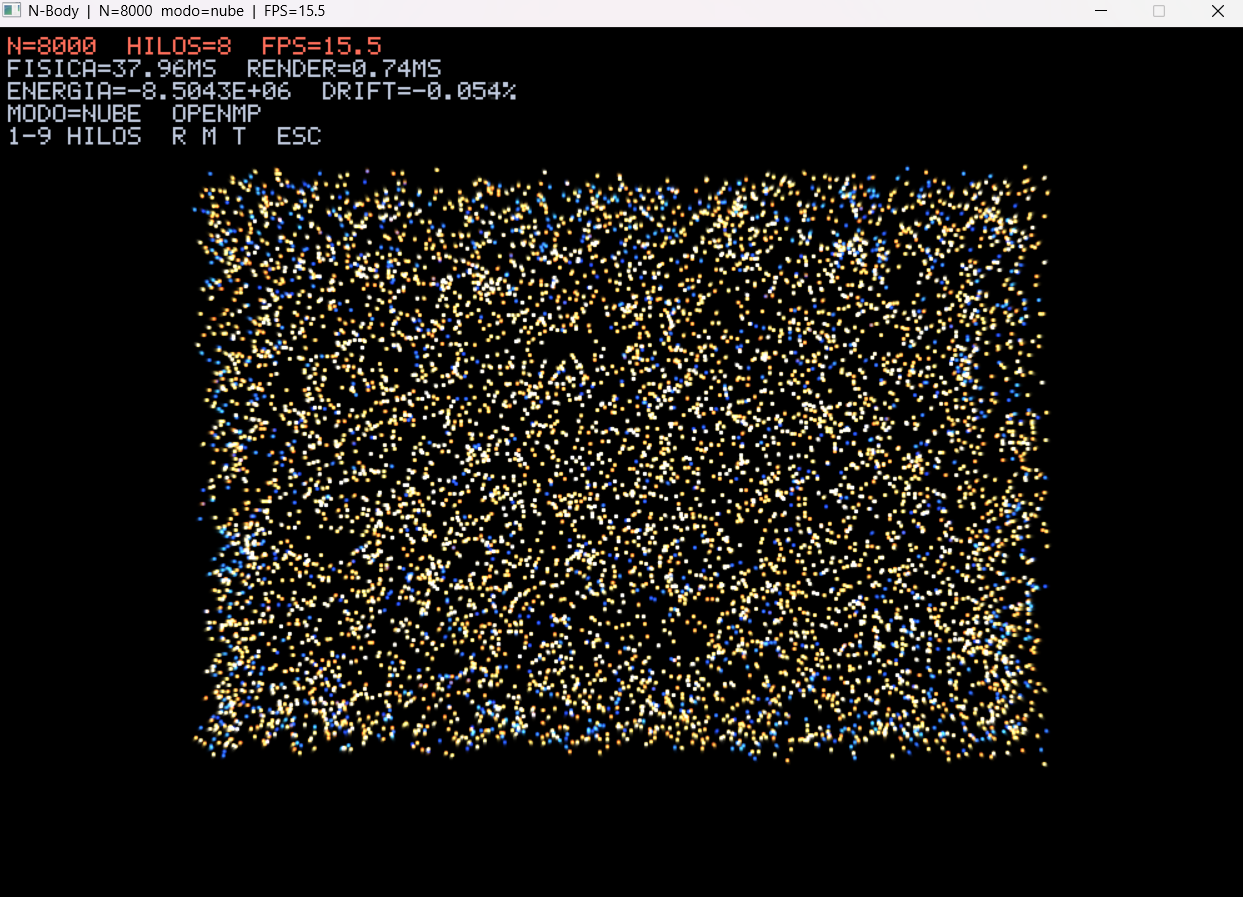
\includegraphics[width=0.85\textwidth]{img/fig3_nube.png}
\caption{Escenario de nube con 8000 cuerpos y 8 hilos}
\end{figure}

\clearpage
\subsection{Estructura de los datos}

Las posiciones, velocidades, aceleraciones, masas y variaciones de color se almacenan
en arreglos separados. Esta organización permite recorrer de manera continua un mismo
atributo para todos los cuerpos y facilita el acceso a memoria durante los ciclos
principales.

La generación pseudoaleatoria utiliza Xorshift32. El estado de este generador no
depende de una variable global compartida. La semilla permite reproducir la misma
configuración inicial cuando se utiliza el mismo valor.

\subsection{Renderizado y panel de métricas}

SDL2 se utiliza para crear la ventana, el renderer y la textura que presenta el
framebuffer en pantalla [4]. El framebuffer utiliza el formato ARGB8888.

Cuando las estelas están activadas, el contenido anterior no se elimina de inmediato.
Los píxeles disminuyen su intensidad y dejan un rastro del movimiento. Los cuerpos se
dibujan mediante pequeños destellos con suma de brillo.

El panel superior muestra la cantidad de cuerpos, la cantidad de hilos, los FPS, el
tiempo de física, el tiempo de renderizado, la energía, la variación de energía y el
modo actual. También indica si la aplicación fue compilada con OpenMP.

\begin{figure}[h!]
\centering
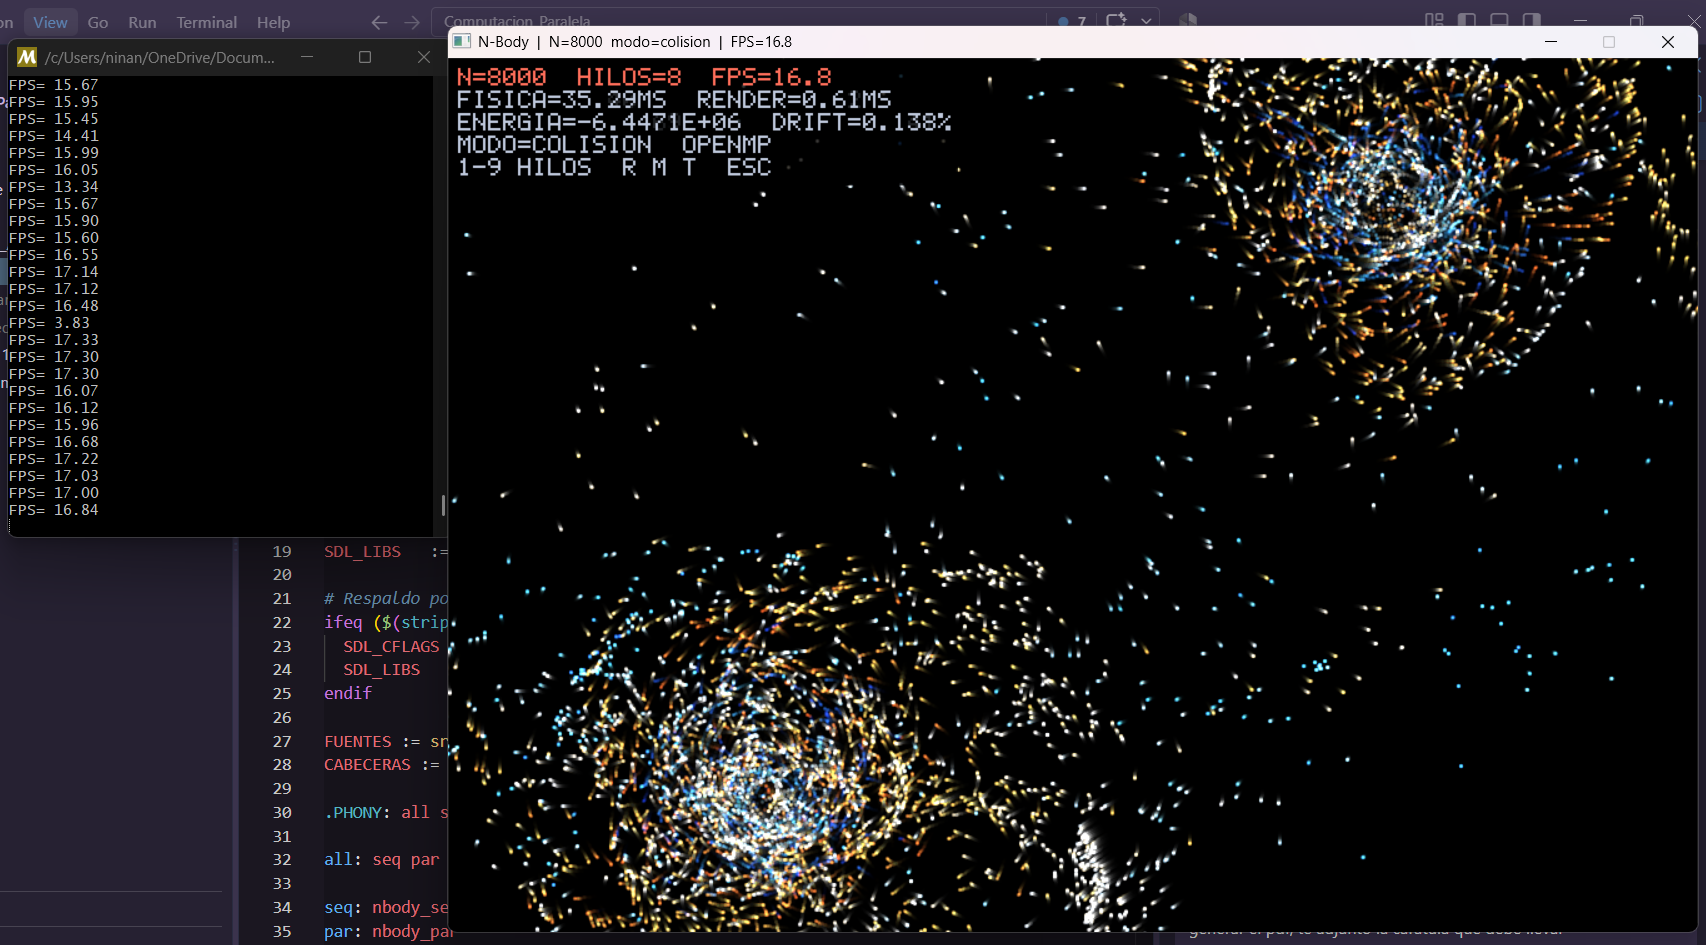
\includegraphics[width=0.9\textwidth]{img/fig4_paralela.png}
\caption{Ejecución de la versión paralela y despliegue de métricas}
\end{figure}

% ---------------------------------------------------------- paralelizacion
\clearpage
\section{Estrategia de paralelización}

\subsection{Partición}

El cálculo de aceleraciones es la parte principal de la simulación. Para cada cuerpo
se recorren todos los demás cuerpos. La iteración externa se divide entre varios hilos
porque cada iteración escribe únicamente la aceleración correspondiente a su propio
índice.

La integración también se divide entre hilos. Cada iteración actualiza la velocidad y
la posición de un solo cuerpo. El desvanecimiento del framebuffer se paraleliza por
píxel porque cada posición de la imagen puede procesarse de forma independiente.

El dibujo de cuerpos requiere una estrategia diferente. Dos cuerpos pueden intentar
modificar el mismo píxel. Para evitar esta condición de carrera, el framebuffer se
divide en bandas horizontales. Cada hilo escribe únicamente en las filas que le
pertenecen.

\subsection{Comunicación}

Durante el cálculo de aceleraciones, las posiciones y las masas son compartidas
únicamente para lectura. Cada hilo utiliza acumuladores locales para calcular la
aceleración de los cuerpos que le corresponden.

Para los cálculos de energía se utilizan reducciones de OpenMP. Cada hilo mantiene un
resultado parcial y OpenMP combina los resultados al finalizar la región paralela.

\subsection{Aglomeración}

El cálculo de aceleraciones utiliza \texttt{schedule runtime}. Esto permite elegir la
política de reparto desde la línea de comandos con \texttt{static}, \texttt{dynamic} o
\texttt{guided}.

Para la bitácora final de rendimiento se utilizó la política \texttt{dynamic}. De esta
forma, las iteraciones se entregan a los hilos conforme estos terminan trabajo previo.
La misma política y los mismos parámetros se mantuvieron en todas las configuraciones
de la prueba para que la comparación entre cantidades de hilos fuera consistente.

\subsection{Mapeo}

OpenMP distribuye las iteraciones entre los hilos disponibles. La cantidad de hilos
puede establecerse con la bandera \texttt{-t}. El valor cero permite que OpenMP
seleccione la cantidad disponible.

Durante la ejecución gráfica también es posible cambiar la cantidad de hilos con las
teclas del 1 al 9. Esto permite observar el efecto de la cantidad de hilos sin
reiniciar el programa.

\subsection{Sincronización}

El programa separa el cálculo de aceleraciones y la integración en dos fases. Al
terminar el ciclo paralelo de aceleraciones existe una barrera implícita de OpenMP. La
integración comienza únicamente cuando todas las aceleraciones ya fueron calculadas.

Esta separación evita que un hilo modifique una posición mientras otro hilo todavía
necesita leer el valor anterior. En el renderizado, la división por bandas evita la
escritura concurrente sobre los mismos píxeles sin utilizar secciones críticas ni
operaciones atómicas.

% --------------------------------------------------------------- defensiva
\section{Programación defensiva y manejo de recursos}

El programa valida los argumentos antes de inicializar SDL2 o reservar los recursos
gráficos. Los valores numéricos se comprueban para asegurar que tengan el tipo
correcto y que se encuentren dentro de los rangos permitidos.

La cantidad de cuerpos, las dimensiones del canvas, la cantidad de hilos, la gravedad,
el suavizado y el paso de tiempo tienen límites definidos. Las opciones desconocidas
generan un mensaje de error y terminan la ejecución de forma controlada.

El suavizado tiene un mínimo de 0.001. Además, el cálculo de aceleraciones mantiene un
valor mínimo interno para evitar divisiones que puedan generar valores no numéricos.

La reserva del sistema y del framebuffer se encuentra dentro de un bloque que captura
errores de memoria insuficiente. Los recursos de SDL2 se agrupan en una estructura que
destruye la textura, el renderer y la ventana al terminar la ejecución.

Antes de convertir posiciones a coordenadas enteras, el renderizado verifica que sean
valores finitos y representables. Los cuerpos que se encuentran demasiado lejos del
canvas no se dibujan.

% -------------------------------------------------------------- compilacion
\section{Compilación y ejecución}

El proyecto utiliza C++17, SDL2 y OpenMP. El archivo \texttt{Makefile} genera las dos
versiones a partir de los mismos archivos fuente.

\begin{table}[h!]
\centering
\caption{Versiones generadas por el proyecto}
\begin{tabular}{|L{4cm}|L{9.5cm}|}
\hline
\textbf{Ejecutable} & \textbf{Descripción} \\
\hline
\texttt{nbody\_seq} & Versión secuencial compilada sin OpenMP. \\
\hline
\texttt{nbody\_par} & Versión paralela compilada con OpenMP. \\
\hline
\end{tabular}
\end{table}

Para compilar ambas versiones se utiliza:

\texttt{make}

Un ejemplo de ejecución paralela es:

\texttt{./nbody\_par.exe -n 8000 -m colision -t 8}

El modo de benchmark ejecuta la física y el renderizado en memoria sin abrir una
ventana. De esta manera se evita incluir el costo de presentación de SDL2 en las
mediciones.

\texttt{./nbody\_par.exe -{}-bench -n 8000 -t 8 -f 50}

% --------------------------------------------------------------- resultados
\section{Resultados y análisis}

\subsection{Resultados de la ejecución visual}

Las capturas de los tres escenarios muestran una ejecución con 8000 cuerpos y 8 hilos.
En las imágenes se observan valores cercanos a 15 y 17 FPS. Estos valores corresponden
al modo interactivo y no deben compararse directamente con el benchmark sin ventana,
ya que la ejecución visual también realiza actualización de textura, presentación y
manejo de eventos.

En las capturas también se observa que el tiempo de física es considerablemente mayor
que el tiempo de renderizado. Esto coincide con la estructura del algoritmo, donde el
cálculo de interacciones entre cuerpos concentra la mayor parte del trabajo.

\subsection{Configuración de la prueba de rendimiento}

La prueba final se ejecutó en modo colisión con la política \texttt{dynamic}. Se
evaluaron dos tamaños de problema, 4000 y 8000 cuerpos. Para cada tamaño se midió la
versión secuencial y la versión paralela con 1, 2, 4 y 8 hilos.

Cada configuración se ejecutó 10 veces y cada repetición midió 20 frames después del
calentamiento. En total se obtuvieron 100 mediciones. Los valores presentados en la
siguiente tabla corresponden al promedio de las 10 repeticiones de cada configuración.

\begin{table}[h!]
\centering
\caption{Resultados promedio del benchmark}
\begin{tabular}{|c|l|c|r|r|r|r|}
\hline
\textbf{N} & \textbf{Versión} & \textbf{Hilos} & \textbf{ms/frame} & \textbf{FPS} &
\textbf{Speedup} & \textbf{Eficiencia} \\
\hline
4000 & Secuencial & 1 & 15.149 & 66.2 & 1.00x & -- \\
\hline
4000 & Paralela & 1 & 29.892 & 33.5 & 0.50x & 50 \% \\
\hline
4000 & Paralela & 2 & 16.104 & 62.4 & 0.93x & 46 \% \\
\hline
4000 & Paralela & 4 & 9.855 & 101.9 & 1.52x & 38 \% \\
\hline
4000 & Paralela & 8 & 8.519 & 117.5 & 1.75x & 22 \% \\
\hline
8000 & Secuencial & 1 & 58.745 & 17.0 & 1.00x & -- \\
\hline
8000 & Paralela & 1 & 131.675 & 7.7 & 0.45x & 45 \% \\
\hline
8000 & Paralela & 2 & 71.746 & 14.0 & 0.82x & 41 \% \\
\hline
8000 & Paralela & 4 & 44.808 & 22.6 & 1.33x & 33 \% \\
\hline
8000 & Paralela & 8 & 42.649 & 23.6 & 1.38x & 17 \% \\
\hline
\end{tabular}
\end{table}

El speedup de la fila secuencial es 1.00x por definición, ya que es la referencia
contra la que se comparan las demás configuraciones del mismo tamaño de problema.

\subsection{Análisis del speedup y la eficiencia}

El speedup compara el tiempo de la versión secuencial con el tiempo de la versión
paralela:

\begin{equation}
S_p = \frac{T_s}{T_p}
\end{equation}

La eficiencia relaciona el speedup con la cantidad de hilos utilizados:

\begin{equation}
E_p = \frac{S_p}{p}
\end{equation}

Con 4000 cuerpos, la versión paralela comienza a superar a la secuencial a partir de 4
hilos. Con 4 hilos alcanza un speedup promedio de 1.52 y con 8 hilos llega a 1.75.
Esto reduce el tiempo promedio por frame de 15.149 ms en la versión secuencial a 8.519
ms con 8 hilos.

Con 8000 cuerpos ocurre un comportamiento similar. La versión paralela con 1 y 2 hilos
resulta más lenta que la versión secuencial, mientras que con 4 y 8 hilos sí se
obtiene aceleración. El mayor speedup medido fue de 1.38 con 8 hilos.

\subsubsection*{Por qué la versión paralela con un hilo es más lenta}

La versión paralela con un solo hilo presenta un tiempo mayor que la versión
secuencial. La causa no es el costo de crear y administrar regiones paralelas: entrar
a una región paralela con un solo hilo cuesta del orden de microsegundos, mientras que
la diferencia medida es de aproximadamente 73 ms por frame con 8000 cuerpos, es decir
unas mil veces mayor.

La causa real es que al compilar con \texttt{-fopenmp} el compilador traslada el
cuerpo de la región paralela a una función generada internamente, y en ese contexto el
vectorizador de GCC deja de procesar el ciclo interno. Esto se comprueba con la opción
de diagnóstico \texttt{-fopt-info-vec}, que reporta:

\begin{quote}
\ttfamily\footnotesize
sin \mbox{-fopenmp}: loop vectorized using 32 byte vectors and unroll factor 8\\
con \mbox{-fopenmp}: not vectorized: unsupported control flow in loop
\end{quote}

Sin vectorización cada hilo procesa un par de cuerpos por instrucción en lugar de
ocho, lo que explica que el rendimiento por hilo se reduzca aproximadamente a la
mitad. Por esta razón la versión paralela necesita alrededor de tres hilos únicamente
para recuperar el rendimiento que pierde al compilarse, y comienza a superar a la
versión secuencial a partir de cuatro hilos.

Se evaluaron cuatro alternativas para recuperar la vectorización: la directiva
\texttt{omp simd} sobre el ciclo interno, extraer el ciclo a una función
independiente, devolver el resultado por valor en lugar de por referencia, y aplicar
bloqueo de registros procesando varios cuerpos a la vez. Las cuatro empeoraron el
tiempo absoluto respecto a la forma actual, por lo que se conservó la versión más
rápida de las medidas.

\subsubsection*{Comportamiento de la eficiencia}

La eficiencia disminuye al aumentar la cantidad de hilos. Para 4000 cuerpos pasa de
aproximadamente 50 por ciento con un hilo paralelo a 22 por ciento con 8 hilos. Para
8000 cuerpos disminuye de aproximadamente 45 por ciento a 17 por ciento. Esto indica
que el speedup no crece de forma proporcional al número de hilos debido al costo de
administración, sincronización y otras partes del programa que no se aceleran en la
misma proporción.

Los resultados también muestran que 4 hilos ofrecen un mejor balance entre aceleración
y eficiencia. En 4000 cuerpos se obtiene un speedup de 1.52 con una eficiencia de 38
por ciento. En 8000 cuerpos se obtiene un speedup de 1.33 con una eficiencia de 33 por
ciento. El uso de 8 hilos entrega el mayor speedup, pero con una disminución
considerable de eficiencia.

% -------------------------------------------------------------- conclusiones
\section{Conclusiones}

La simulación de N cuerpos es adecuada para aplicar paralelización porque el cálculo
de aceleraciones contiene una gran cantidad de operaciones independientes. Cada
iteración externa puede asignarse a un hilo distinto sin modificar las posiciones que
los demás hilos están leyendo.

La separación entre el cálculo de aceleraciones y la integración permite mantener un
estado consistente durante cada paso. La barrera implícita de OpenMP asegura que todas
las aceleraciones estén listas antes de actualizar posiciones y velocidades.

La estrategia de dividir el framebuffer en bandas horizontales permite paralelizar el
dibujo sin producir condiciones de carrera sobre los píxeles. Cada hilo trabaja
únicamente dentro de su propia región de la imagen.

Las 100 mediciones realizadas muestran que la paralelización sí mejora el rendimiento
cuando se utilizan suficientes hilos. Para 4000 cuerpos el mejor resultado fue de
117.5 FPS y un speedup de 1.75 con 8 hilos. Para 8000 cuerpos el mejor resultado fue
de 23.6 FPS y un speedup de 1.38 también con 8 hilos.

La versión paralela con 1 y 2 hilos no supera a la versión secuencial en las pruebas
realizadas. Esto se debe a la pérdida de vectorización que introduce la compilación
con OpenMP, y demuestra que utilizar más hilos no garantiza por sí solo una mejora de
rendimiento.

La eficiencia disminuye conforme aumenta la cantidad de hilos. Por esta razón, 4 hilos
presentan un mejor balance entre aceleración y aprovechamiento de los recursos,
mientras que 8 hilos permiten obtener el mayor speedup medido.

% ----------------------------------------------------------- recomendaciones
\section{Recomendaciones}

Se recomienda realizar las mediciones de rendimiento con la menor cantidad posible de
aplicaciones adicionales en ejecución. Esto ayuda a reducir variaciones provocadas por
otros procesos del sistema.

También se recomienda utilizar la misma semilla, el mismo escenario, la misma cantidad
de frames y los mismos parámetros físicos cuando se comparan distintas cantidades de
hilos. De esta manera, las configuraciones realizan una carga de trabajo equivalente.

Para comparar el desempeño se recomienda utilizar el modo \texttt{-{}-bench}, ya que
mide la física y el renderizado sin incluir el costo de mostrar la ventana. La
ejecución visual puede utilizarse como evidencia del funcionamiento y para observar
los FPS desde el punto de vista del usuario.

Si se busca el mayor rendimiento de las configuraciones evaluadas, 8 hilos ofrecen el
mayor speedup. Si se busca un mejor equilibrio entre speedup y eficiencia, los
resultados indican que 4 hilos son una opción más conveniente.

Como trabajo futuro se recomienda investigar formas de conservar la vectorización del
ciclo interno bajo OpenMP, ya que recuperar ese factor duplicaría el rendimiento de
todas las configuraciones paralelas sin necesidad de utilizar más hilos.

% ------------------------------------------------------------- referencias
\section*{Referencias}
\addcontentsline{toc}{section}{Referencias}

\begin{enumerate}
\item[{[1]}] OpenMP Architecture Review Board. \emph{OpenMP Application Programming
Interface Version 5.2}. 2021. \url{https://www.openmp.org/specifications/}
\item[{[2]}] Ian Foster. \emph{Designing and Building Parallel Programs}.
Addison-Wesley. 1995.
\item[{[3]}] Sverre J. Aarseth. \emph{Gravitational N-Body Simulations: Tools and
Algorithms}. Cambridge University Press. 2003.
\item[{[4]}] Simple DirectMedia Layer. \emph{SDL2 Documentation}.
\url{https://wiki.libsdl.org/SDL2/FrontPage}
\end{enumerate}

% ----------------------------------------------------------------- anexo 1
\appendix
\section{Anexo 1. Diagrama de flujo del programa}

El diagrama resume la captura de argumentos, la validación de entradas, la
configuración de OpenMP, la reserva de recursos, las secciones paralelas, la
sincronización, el renderizado, el despliegue de resultados y la liberación de
recursos.

\begin{figure}[h!]
\centering
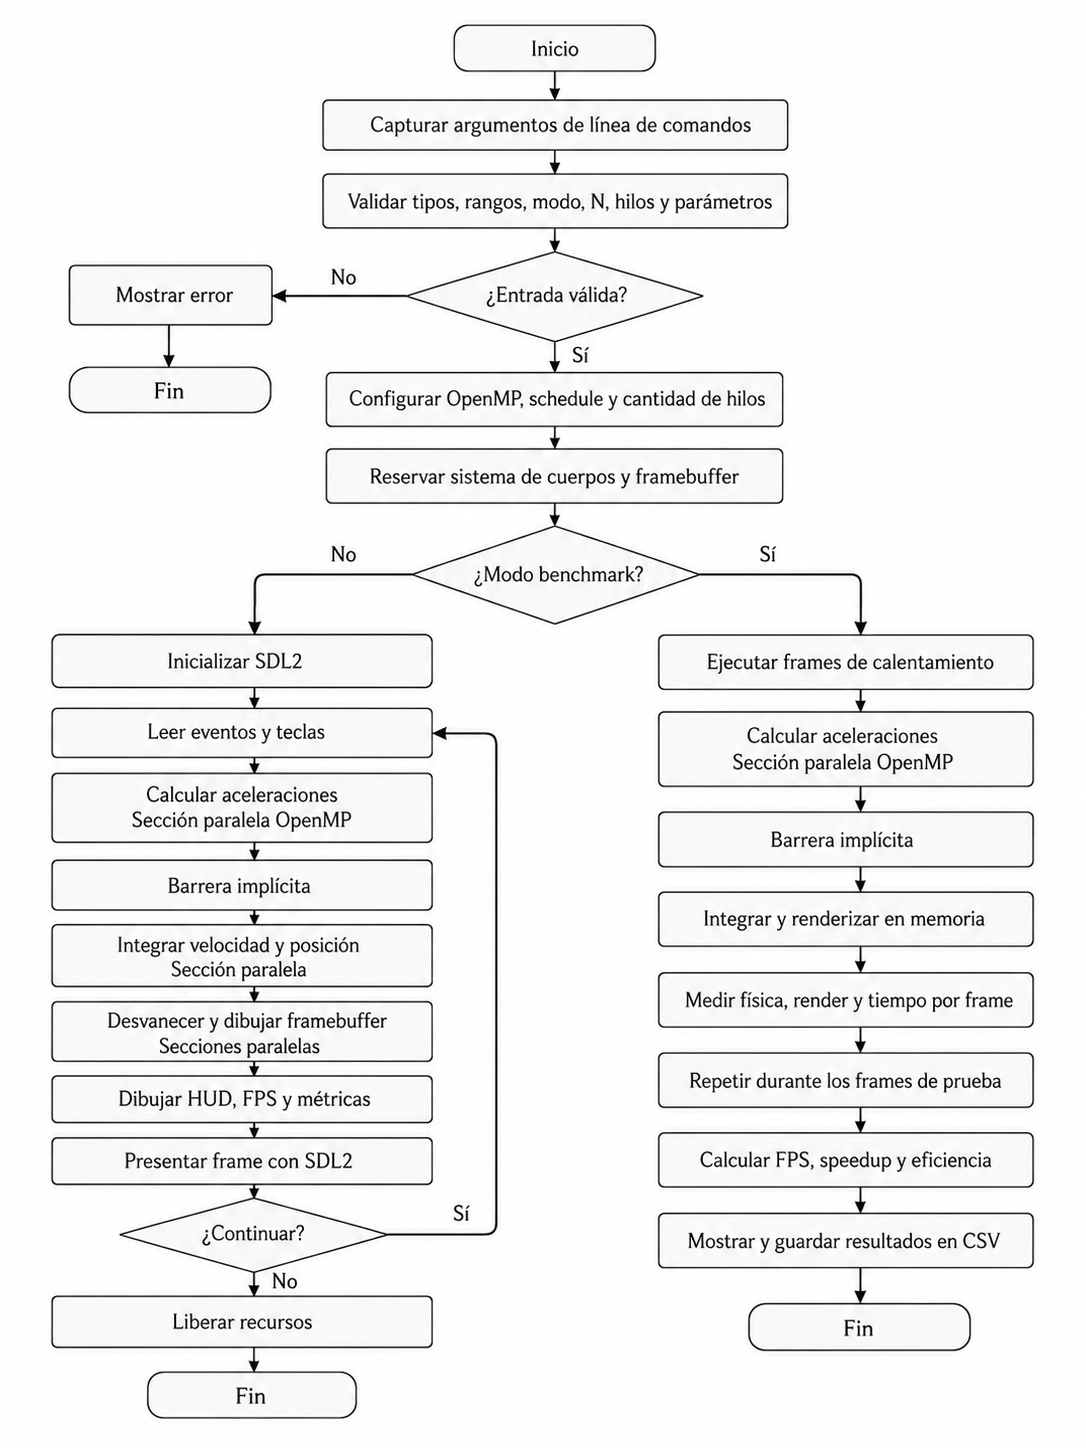
\includegraphics[width=0.95\textwidth]{img/fig5_diagrama.png}
\caption{Diagrama de flujo general del programa}
\end{figure}

% ----------------------------------------------------------------- anexo 2
\clearpage
\begin{landscape}
\section{Anexo 2. Catálogo de funciones}

Para cada función se indican los parámetros de entrada con su nombre y tipo exactos,
el tipo de retorno y el propósito de la rutina. Las funciones miembro de
\texttt{SistemaNCuerpos} no reciben parámetros: operan sobre los arreglos internos del
objeto, por lo que se indica cuáles arreglos leen y cuáles escriben.

\footnotesize
% tabcolsep reducido: con el valor por defecto (6pt) los ocho separadores se
% comen 1.7cm y la tabla no cabe en el ancho apaisado.
\setlength{\tabcolsep}{3pt}
\begin{longtable}{|M{4.3cm}|L{7.0cm}|L{3.8cm}|L{6.8cm}|}
\hline
\textbf{\normalfont Función o rutina} & \textbf{Entradas (nombre y tipo)} &
\textbf{Salida} & \textbf{Descripción} \\
\hline
\endfirsthead
\hline
\textbf{\normalfont Función o rutina} & \textbf{Entradas (nombre y tipo)} &
\textbf{Salida} & \textbf{Descripción} \\
\hline
\endhead
\hline
\endfoot

\multicolumn{4}{|l|}{\normalfont\textbf{cli.cpp / cli.h --- argumentos y validación}} \\
\hline

a\_long &
\texttt{const std::string\& texto}, \texttt{long\& out} &
\texttt{bool} &
Convierte texto a entero largo. Devuelve falso si el texto está vacío, si sobra
basura al final o si hay desbordamiento. \\
\hline

a\_double &
\texttt{const std::string\& texto}, \texttt{double\& out} &
\texttt{bool} &
Convierte texto a un valor real y comprueba errores de conversión. \\
\hline

siguiente\_valor &
\texttt{int argc}, \texttt{char** argv}, \texttt{int\& i},
\texttt{std::string\& out} &
\texttt{bool} &
Obtiene el valor que sigue a una bandera. Devuelve falso si la bandera venía al final
de la línea sin valor. \\
\hline

leer\_entero &
\texttt{int argc}, \texttt{char** argv}, \texttt{int\& i},
\texttt{const std::string\& bandera}, \texttt{long lo}, \texttt{long hi},
\texttt{long\& out} &
\texttt{bool} &
Lee un entero y comprueba que se encuentre en el intervalo cerrado
$[\mathtt{lo}, \mathtt{hi}]$. \\
\hline

leer\_real &
\texttt{int argc}, \texttt{char** argv}, \texttt{int\& i},
\texttt{const std::string\& bandera}, \texttt{double lo}, \texttt{double hi},
\texttt{double\& out} &
\texttt{bool} &
Lee un valor real y comprueba que se encuentre en el intervalo
$(\mathtt{lo}, \mathtt{hi}]$, abierto por abajo. \\
\hline

reparto\_desde\_texto &
\texttt{const std::string\& texto}, \texttt{Reparto\& out} &
\texttt{bool} &
Convierte \texttt{static}, \texttt{dynamic} o \texttt{guided} al tipo interno
\texttt{Reparto}. \\
\hline

texto\_de\_reparto &
\texttt{Reparto r} &
\texttt{const char*} &
Devuelve el nombre de la política de reparto, para el CSV y los mensajes de error. \\
\hline

imprimir\_ayuda &
\texttt{const char* nombre\_programa} &
\texttt{void} &
Muestra las banderas disponibles, sus rangos, las teclas y ejemplos de uso. \\
\hline

parsear\_argumentos &
\texttt{int argc}, \texttt{char** argv}, \texttt{Parametros\& out} &
\texttt{bool} &
Procesa y valida toda la configuración de la línea de comandos. Devuelve falso ante
cualquier entrada inválida. \\
\hline

\multicolumn{4}{|l|}{\normalfont\textbf{nbody.cpp / nbody.h --- física de la simulación}} \\
\hline

modo\_desde\_texto &
\texttt{const std::string\& texto}, \texttt{Modo\& out} &
\texttt{bool} &
Convierte \texttt{colision}, \texttt{galaxia} o \texttt{nube} al tipo interno
\texttt{Modo}. \\
\hline

texto\_de\_modo &
\texttt{Modo m} &
\texttt{const char*} &
Devuelve el nombre del escenario actual. \\
\hline

SistemaNCuerpos (constructor) &
\texttt{int n}, \texttt{int ancho}, \texttt{int alto}, \texttt{Modo modo},
\texttt{uint32\_t semilla}, \texttt{const ParametrosFisica\& fisica} &
Objeto construido &
Reserva los ocho arreglos internos de tamaño \texttt{n} y siembra el escenario. Lanza
\texttt{std::bad\_alloc} si \texttt{n} no cabe en memoria. \\
\hline

sembrar\_disco &
\texttt{Xorshift32\& r}, \texttt{int desde}, \texttt{int cuenta},
\texttt{float cx}, \texttt{float cy}, \texttt{float vx\_bulk},
\texttt{float vy\_bulk}, \texttt{int giro} &
\texttt{void} &
Crea un disco galáctico con núcleo masivo en el índice \texttt{desde} y estrellas en
órbita circular. \texttt{giro} vale $+1$ o $-1$. \\
\hline

sembrar\_nube &
\texttt{Xorshift32\& r} &
\texttt{void} &
Distribuye los cuerpos de forma pseudoaleatoria con masas iguales y velocidades
iniciales pequeñas. \\
\hline

reiniciar &
\texttt{Modo modo}, \texttt{uint32\_t semilla} &
\texttt{void} &
Vuelve a sembrar el escenario sin reasignar los arreglos. \\
\hline

calcular\_aceleraciones &
Sin parámetros. Lee \texttt{px\_}, \texttt{py\_}, \texttt{masa\_}
(\texttt{std::vector<float>}); escribe \texttt{ax\_}, \texttt{ay\_} &
\texttt{void} &
Calcula la aceleración gravitacional de cada cuerpo. El ciclo externo se paraleliza
con \texttt{schedule(runtime)}. \\
\hline

integrar &
Sin parámetros. Lee \texttt{ax\_}, \texttt{ay\_}; escribe \texttt{vx\_},
\texttt{vy\_}, \texttt{px\_}, \texttt{py\_} (\texttt{std::vector<float>}) &
\texttt{void} &
Actualiza velocidad y posición mediante Euler semiimplícito, tras la barrera
implícita. \\
\hline

energia\_cinetica &
Sin parámetros. Lee \texttt{masa\_}, \texttt{vx\_}, \texttt{vy\_}
(\texttt{std::vector<float>}) &
\texttt{double} &
Calcula la energía cinética total usando \texttt{reduction(+:ke)}. \\
\hline

energia\_potencial &
Sin parámetros. Lee \texttt{masa\_}, \texttt{px\_}, \texttt{py\_}
(\texttt{std::vector<float>}) &
\texttt{double} &
Calcula la energía potencial de todos los pares con \texttt{reduction(+:pe)} y
\texttt{schedule(dynamic)}. \\
\hline

n / rapidez\_ref / px / py / vx / vy / tono\_jitter &
Sin parámetros &
\texttt{int}, \texttt{float} y
\texttt{const std::vector<float>\&} &
Acceso de solo lectura al tamaño, la escala de color y los arreglos internos, para el
renderizado. \\
\hline

\multicolumn{4}{|l|}{\normalfont\textbf{rng.h --- generador pseudoaleatorio}} \\
\hline

Xorshift32 (constructor) &
\texttt{uint32\_t semilla} &
Objeto construido &
Inicializa el generador y evita el estado cero, que se quedaría bloqueado. \\
\hline

siguiente &
Sin parámetros. Usa \texttt{estado} (\texttt{uint32\_t}) &
\texttt{uint32\_t} &
Produce el siguiente valor pseudoaleatorio y actualiza el estado privado. \\
\hline

uniforme01 &
Sin parámetros &
\texttt{float} &
Produce un valor pseudoaleatorio en el intervalo $[0, 1)$. \\
\hline

rango &
\texttt{float lo}, \texttt{float hi} &
\texttt{float} &
Produce un valor pseudoaleatorio en $[\mathtt{lo}, \mathtt{hi})$. \\
\hline

\multicolumn{4}{|l|}{\normalfont\textbf{palette.cpp --- color}} \\
\hline

mezclar &
\texttt{uint8\_t a}, \texttt{uint8\_t b}, \texttt{float f} &
\texttt{uint8\_t} &
Interpola linealmente entre dos valores de un canal de color. \\
\hline

color\_por\_rapidez &
\texttt{float t} (rapidez normalizada, se recorta a $[0,1]$) &
\texttt{ColorRGB} &
Obtiene un color de la rampa de cinco paradas: azul, cian, blanco, amarillo y
naranja. \\
\hline

\multicolumn{4}{|l|}{\normalfont\textbf{render.cpp / render.h --- dibujo}} \\
\hline

sumar\_saturando &
\texttt{uint32\_t dst}, \texttt{int r}, \texttt{int g}, \texttt{int b} &
\texttt{uint32\_t} &
Suma brillo a un píxel ARGB8888 sin permitir que un canal exceda 255. \\
\hline

NucleoDestello (constructor) &
Sin parámetros &
Objeto construido &
Precalcula los 25 pesos del destello, una sola vez al arrancar el programa. \\
\hline

desvanecer &
\texttt{std::vector<uint32\_t>\& fb}, \texttt{uint32\_t factor} &
\texttt{void} &
Multiplica cada canal por \texttt{factor/256} para generar las estelas. Ciclo
paralelo por píxel. \\
\hline

limpiar &
\texttt{std::vector<uint32\_t>\& fb}, \texttt{uint32\_t color} &
\texttt{void} &
Rellena todo el framebuffer con un solo color. \\
\hline

dibujar\_cuerpos &
\texttt{std::vector<uint32\_t>\& fb}, \texttt{int ancho}, \texttt{int alto},
\texttt{const SistemaNCuerpos\& sistema},
\texttt{const std::vector<float>\& tono\_jitter} &
\texttt{void} &
Dibuja cada cuerpo como un destello aditivo coloreado por rapidez más el
desplazamiento de tono. Divide el framebuffer en bandas de filas disjuntas para evitar
condiciones de carrera. \\
\hline

\multicolumn{4}{|l|}{\normalfont\textbf{hud.cpp / hud.h --- panel de métricas}} \\
\hline

empacar &
\texttt{uint8\_t r}, \texttt{uint8\_t g}, \texttt{uint8\_t b} &
\texttt{uint32\_t} &
Convierte componentes RGB al formato ARGB8888. \\
\hline

dibujar\_texto &
\texttt{std::vector<uint32\_t>\& fb}, \texttt{int ancho}, \texttt{int alto},
\texttt{int x}, \texttt{int y}, \texttt{const char* texto},
\texttt{uint32\_t color} &
\texttt{void} &
Dibuja una línea de texto con la fuente bitmap 5x7 incluida en el programa. \\
\hline

atenuar\_recuadro &
\texttt{std::vector<uint32\_t>\& fb}, \texttt{int ancho}, \texttt{int alto},
\texttt{int x0}, \texttt{int y0}, \texttt{int w}, \texttt{int h} &
\texttt{void} &
Oscurece el fondo del panel para que el texto se lea sobre cualquier escena. \\
\hline

dibujar\_hud &
\texttt{std::vector<uint32\_t>\& fb}, \texttt{int ancho}, \texttt{int alto},
\texttt{const MetricasHud\& m} &
\texttt{void} &
Dibuja el panel de métricas en la esquina superior izquierda. La línea de FPS se pinta
verde si alcanza 30 y roja si no. \\
\hline

\multicolumn{4}{|l|}{\normalfont\textbf{main.cpp --- ventana, ciclo principal y medición}} \\
\hline

hilos\_activos &
Sin parámetros &
\texttt{int} &
Devuelve la cantidad de hilos configurados en OpenMP, o 1 en la versión secuencial. \\
\hline

fijar\_hilos &
\texttt{int n} &
\texttt{void} &
Establece la cantidad de hilos. Un valor menor o igual a cero deja que OpenMP
decida. \\
\hline

ContextoSDL (destructor) &
Sin parámetros. Opera sobre \texttt{SDL\_Window*}, \texttt{SDL\_Renderer*} y
\texttt{SDL\_Texture*} &
\texttt{void} &
Destruye textura, renderer y ventana, comprobando cada puntero. Cubre también los
fallos a mitad de la inicialización. \\
\hline

iniciar\_sdl &
\texttt{ContextoSDL\& ctx}, \texttt{const Parametros\& p} &
\texttt{bool} &
Inicializa SDL2 y crea ventana, renderer y textura. Cae a renderer por software si no
hay aceleración disponible. \\
\hline

aplicar\_reparto &
\texttt{Reparto r}, \texttt{int trozo} &
\texttt{void} &
Configura la política que utilizará \texttt{schedule(runtime)}. Un trozo de cero deja
que OpenMP elija. \\
\hline

ejecutar\_benchmark &
\texttt{const Parametros\& p} &
\texttt{int} &
Ejecuta el calentamiento, mide física y renderizado por separado y emite una fila CSV.
No inicializa SDL2. \\
\hline

main &
\texttt{int argc}, \texttt{char** argv} &
\texttt{int} &
Coordina validación, configuración, simulación, eventos, métricas y liberación de
recursos. \\
\hline

\end{longtable}
\normalsize
\end{landscape}

% ----------------------------------------------------------------- anexo 3
\clearpage
\section{Anexo 3. Bitácora de pruebas}

La bitácora final se generó mediante el script \texttt{scripts/bench.ps1}. Se
utilizaron 10 repeticiones por configuración y 20 frames medidos por repetición. Se
probaron 4000 y 8000 cuerpos con la versión secuencial y con la versión paralela
utilizando 1, 2, 4 y 8 hilos. El archivo \texttt{bench.csv} contiene un total de 100
mediciones individuales.

El comando utilizado para ejecutar la prueba fue:

\begin{quote}
\ttfamily
.$\backslash$scripts$\backslash$bench.ps1 -Repeticiones 10 -Frames 20\\
-ListaN 4000,8000 -ListaHilos 1,2,4,8
\end{quote}

\begin{table}[h!]
\centering
\caption{Resumen de la bitácora de pruebas}
\begin{tabular}{|c|l|c|c|r|r|r|r|}
\hline
\textbf{N} & \textbf{Versión} & \textbf{Hilos} & \textbf{Reps.} &
\textbf{ms/frame} & \textbf{FPS} & \textbf{Speedup} & \textbf{Eficiencia} \\
\hline
4000 & Secuencial & 1 & 10 & 15.149 & 66.2 & 1.00x & -- \\
\hline
4000 & Paralela & 1 & 10 & 29.892 & 33.5 & 0.50x & 50 \% \\
\hline
4000 & Paralela & 2 & 10 & 16.104 & 62.4 & 0.93x & 46 \% \\
\hline
4000 & Paralela & 4 & 10 & 9.855 & 101.9 & 1.52x & 38 \% \\
\hline
4000 & Paralela & 8 & 10 & 8.519 & 117.5 & 1.75x & 22 \% \\
\hline
8000 & Secuencial & 1 & 10 & 58.745 & 17.0 & 1.00x & -- \\
\hline
8000 & Paralela & 1 & 10 & 131.675 & 7.7 & 0.45x & 45 \% \\
\hline
8000 & Paralela & 2 & 10 & 71.746 & 14.0 & 0.82x & 41 \% \\
\hline
8000 & Paralela & 4 & 10 & 44.808 & 22.6 & 1.33x & 33 \% \\
\hline
8000 & Paralela & 8 & 10 & 42.649 & 23.6 & 1.38x & 17 \% \\
\hline
\end{tabular}
\end{table}

La tabla resume los promedios obtenidos a partir de las 10 repeticiones de cada
configuración. La eficiencia solamente se reporta para la versión paralela, ya que
expresa qué proporción del speedup se obtiene por cada hilo utilizado. El speedup de
las filas secuenciales es 1.00x por definición, al ser la referencia de comparación.

\begin{figure}[h!]
\centering
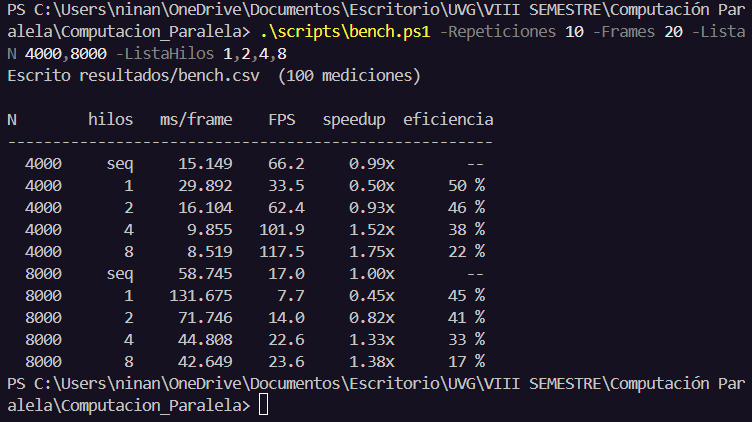
\includegraphics[width=0.95\textwidth]{img/fig6_bench.png}
\caption{Resumen de las 100 mediciones generadas por el benchmark}
\end{figure}

La captura muestra el resumen producido al finalizar el script. En ella se observan el
tiempo promedio por frame, los FPS, el speedup y la eficiencia de cada configuración
evaluada.

\end{document}
